\subsection{ERROR REDUCTION}

In this section, we discuss error of analysis of images. Followed Object can be differents forms. However, 
ROI is rectangular window. We identify certains areas inside of ROI that has more importance than others.

\begin{figure}[H]
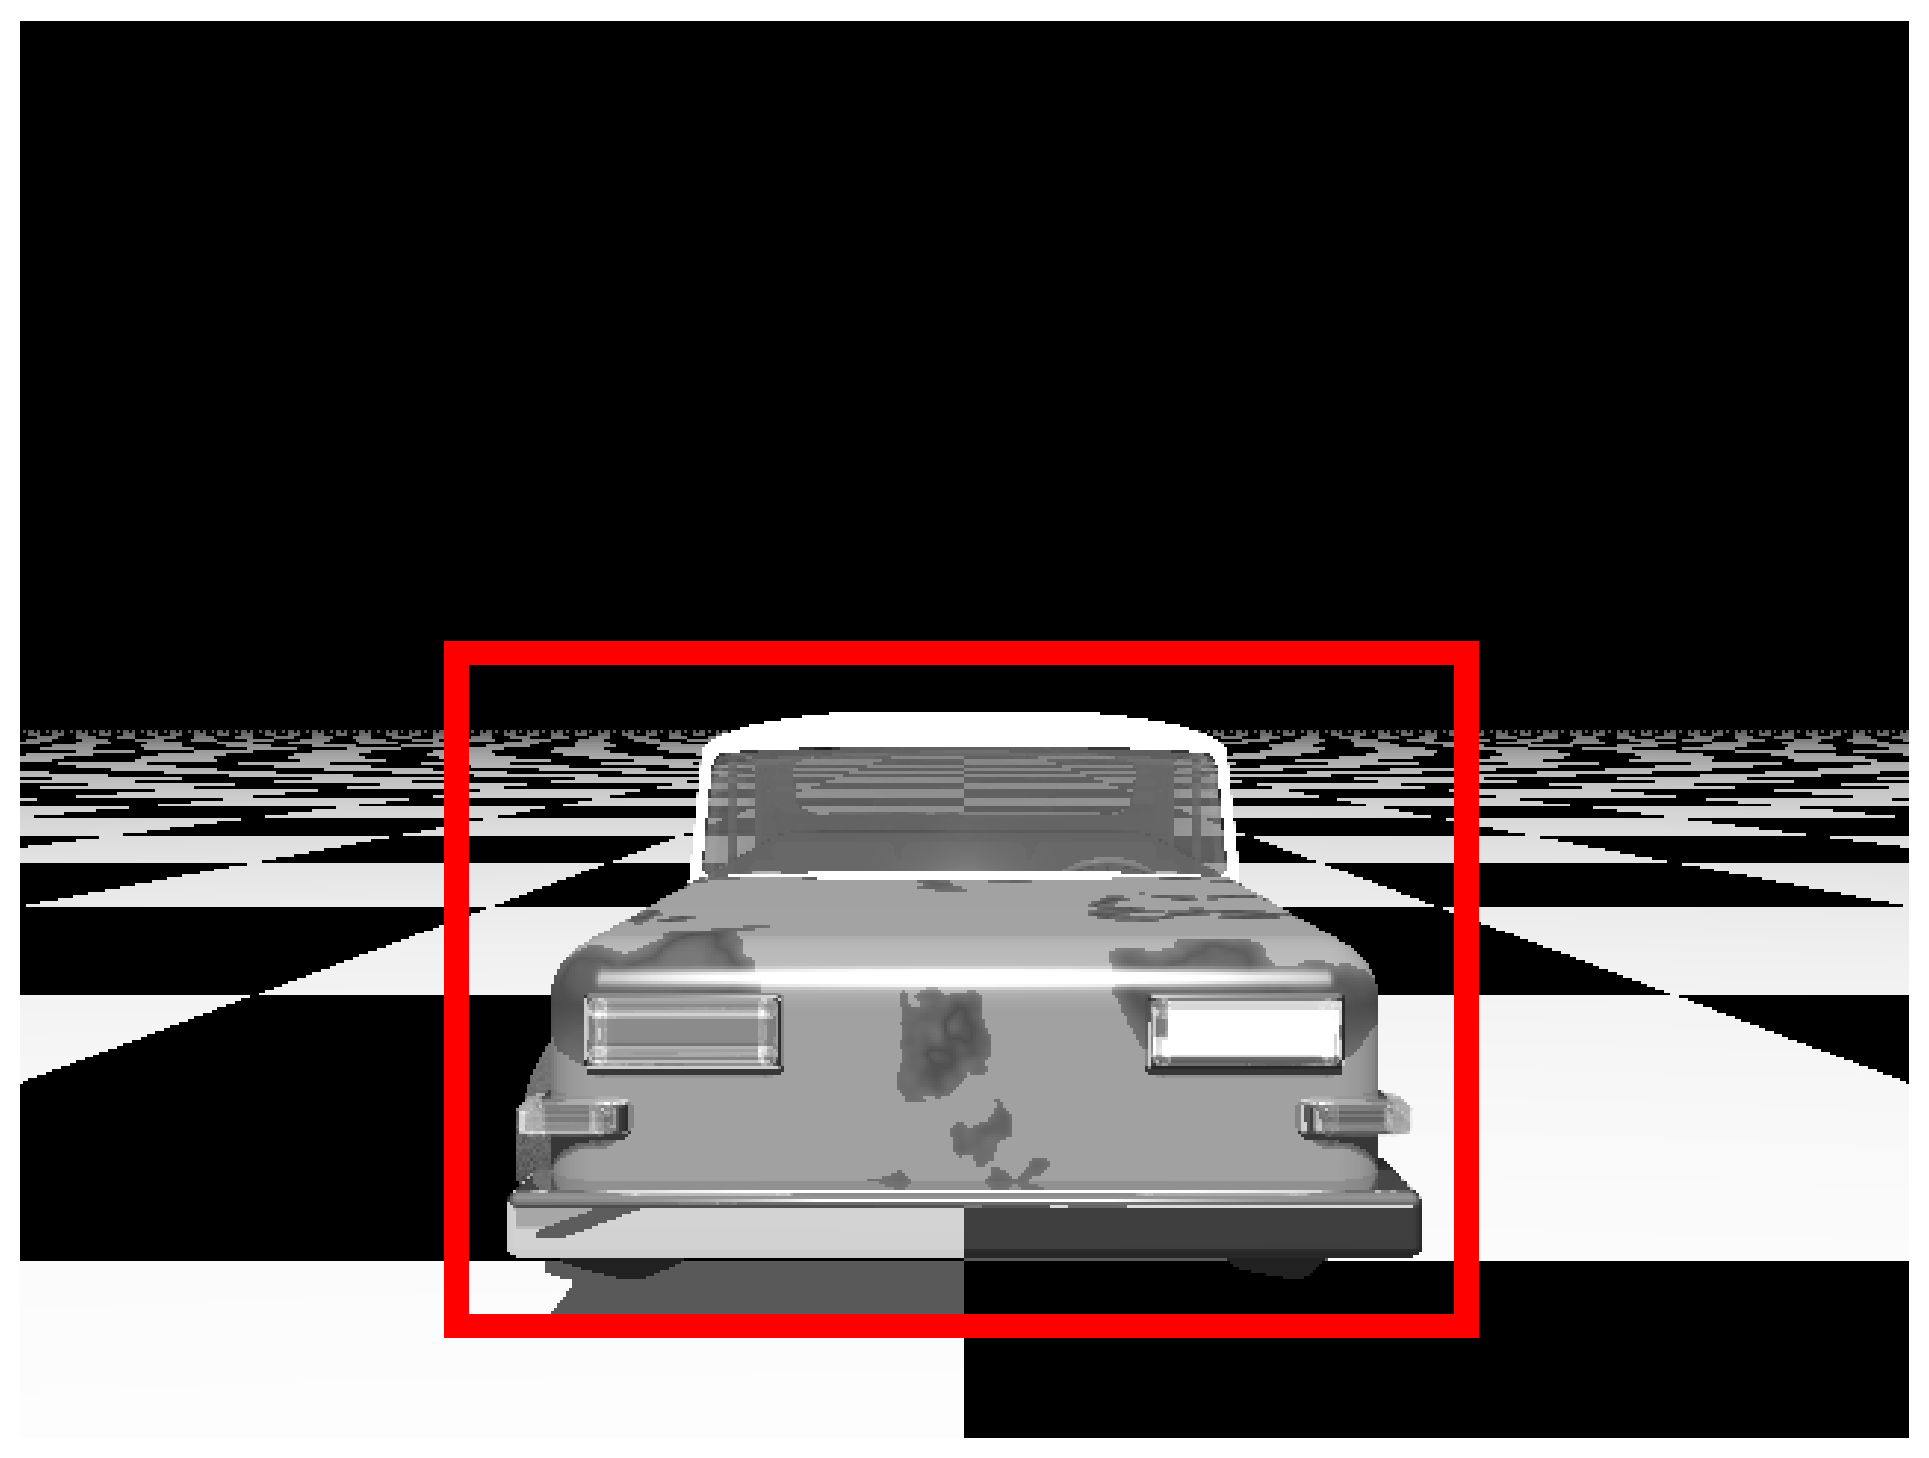
\includegraphics[width=\columnwidth]{images/imageError.eps}
\caption{Illustration of ROI with error close at edges}
\label{fig:erroridentified}
\end{figure}

In Fig. \ref{fig:erroridentified}, there are an error points close of edges because object not occupies whole ROI. The reason of this is
because to do correlation in PCC, we must have two matrix at same dimensios. It's not possible for this kind of correlation 
generate any date with imagens of differents dimensions. However, PCC has high precision in its analysis.

We decide solve this problem given a ponderation in PCC. Then, Points of most importance was considered plus important 
at correlation and given values bigger and points of less importance has low weight at correlation.

\begin{figure}[H]
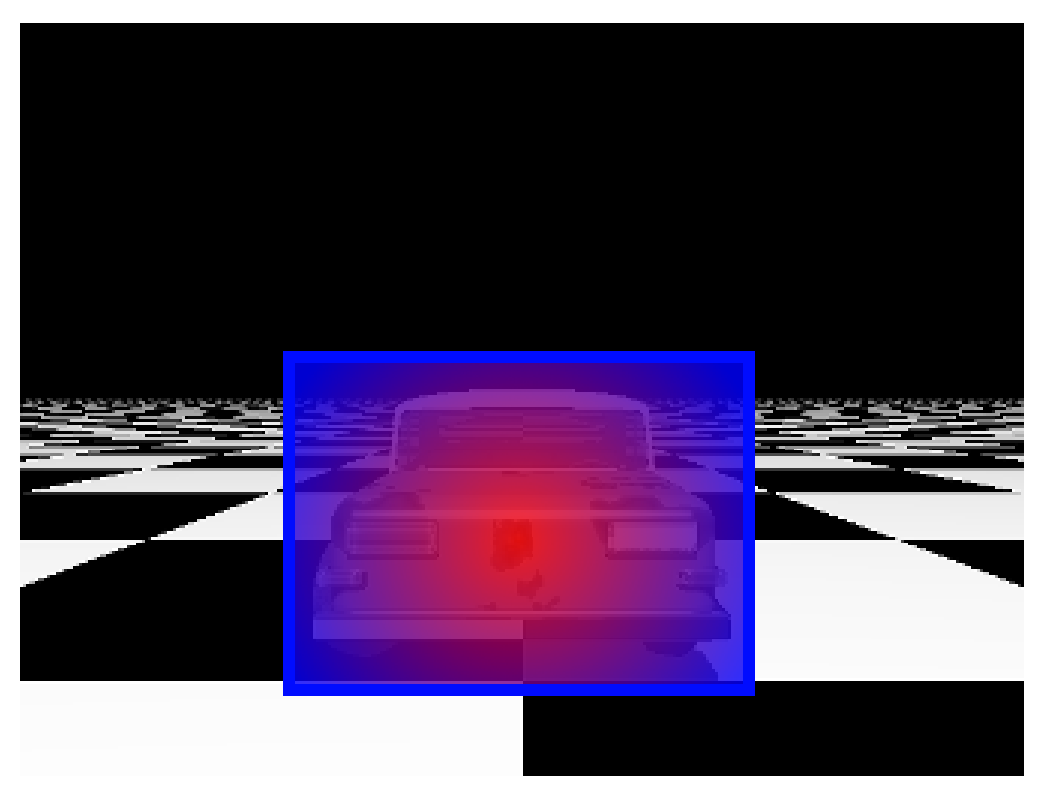
\includegraphics[width=\columnwidth]{images/imageErrorcontroled.eps}
\caption{Illustration of points of most importance (red) and points less importance (blue) in correlation.}
\label{fig:errorpondered}
\end{figure}

Points close of edge, there are less importance and they are in blue at Fig. \ref{fig:errorpondered}. Points close of center of image, 
they are red because object is taken for them.